\documentclass[a4paper, 10pt, final]{article}
\usepackage{michael}

%% \def\mytitle{Signal and Image Processing 2010}
%% \def\mysubtitle{Handin of mandatory excercise 1}
%% \def\myauthor{Ulrik Bonde}
%% \def\mymail{\mailto{bonde@diku.dk}}
%% \def\mydate{\today}

\title{Signal and Image Processing 2010 \\ Mandatory hand-in exercise 2}
\author{Michael Andersen}
\date{\today}

%% \title{\mytitle}
%% \subtitle{\mysubtitle}

%% \author{\myauthor{} - \mymail}
%% \date{\mydate}

\hypersetup{
colorlinks,%
citecolor=black,%
filecolor=black,%
linkcolor=black,%
urlcolor=black,%
bookmarksopen=false,
pdftitle={Signal and Image Processing 2010 - Mandatory exercise 2},
pdfauthor={Michael Andersen}
}

\begin{document}
\maketitle

\subsection*{Question 2.1}
We are to implement a program that performs the fourier transform on
two images. In figure \ref{fig:exercise2_1a} a) we see the original
square, in b) we see the fourier transformed image. Horizontal lines
in a) corresponds to vertical lines in the fourier domain in picture
b). The visible cross within the fourier transformed picture is a
result of the transition \emph{black--white--black}, this results in
high frequencies resulting in the white color.

\begin{figure}[!ht]
\centering
\subfloat[]{
\includegraphics[width=0.4\textwidth]{./images/square}}
\subfloat[]{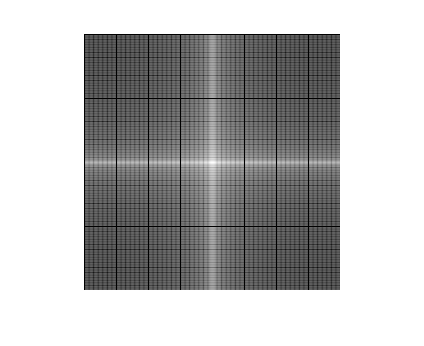
\includegraphics[width=0.4\textwidth]{./images/ft_square}} \\
\subfloat[]{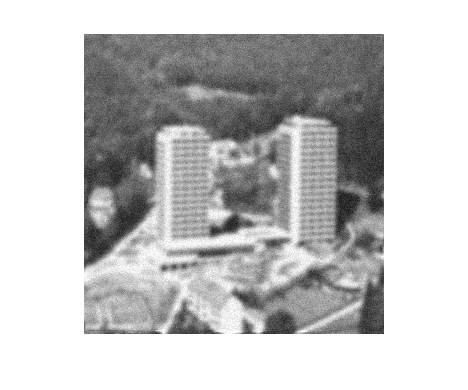
\includegraphics[width=0.4\textwidth]{./images/noisy2}}
\subfloat[]{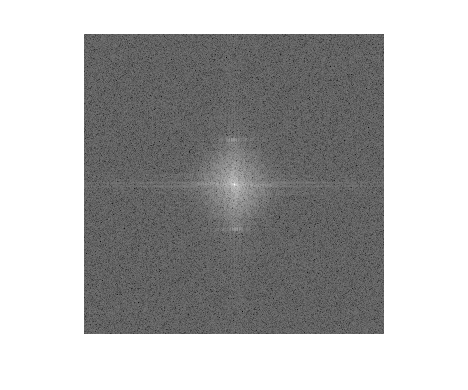
\includegraphics[width=0.4\textwidth]{./images/ft_noisy2}}
\caption{a) Image 1, b) Fourier transform of image 1, c) Image 2, d) Fourier transform of image 2}
\label{fig:exercise2_1a}
\end{figure}

Image 2 in figure \ref{fig:exercise2_1a} is very noisy, this means
that there are not that many instant transitions with the original
image. This results in the fourier transformed image being less
structured and also looking noisy. As the fourier transform is
periodic we see some patterns from wrapping around the original image
edge, where there are some ``rapid'' transitions from light areas to
darker areas.

In figure \ref{fig:exercise2_1b} I have performed padding to
$1024$x$1024$ on both images, the result is apparently is that the
fourier transform seems brighter, which is a result of higher
frequencies, but this should not happen with padding. In image b) in
figure \ref{fig:exercise2_1b} the transition from the noisy picture to
the padding with zeroes is now more visible.

\begin{figure}[!ht]
\centering
\subfloat[]{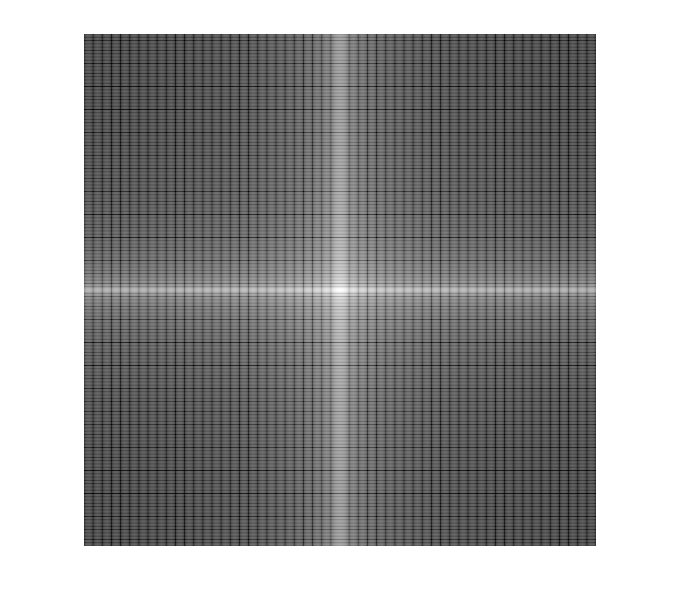
\includegraphics[width=0.4\textwidth]{./images/ft_pad_square}}
\subfloat[]{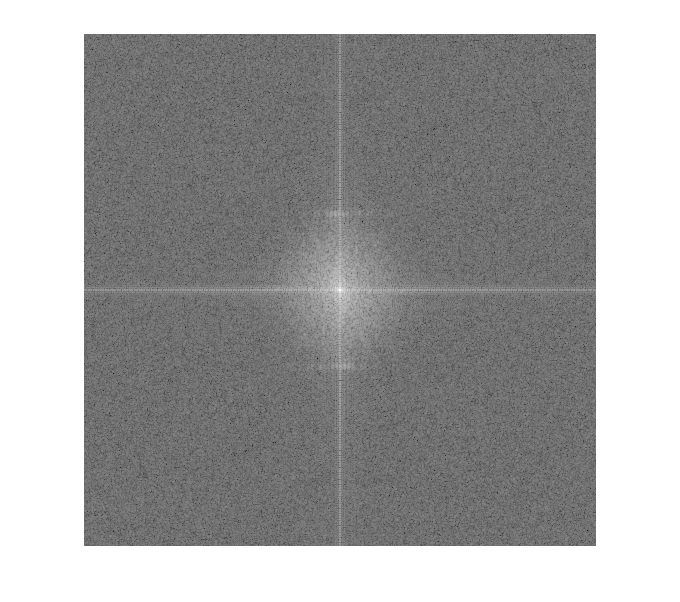
\includegraphics[width=0.4\textwidth]{./images/ft_pad_noisy2}}
\caption{a) Fourier transform with padding of image 1 in figure \ref{fig:exercise2_1a}, b) Fourier transform with padding of image 2 in figure \ref{fig:exercise2_1a} }
\label{fig:exercise2_1b}
\end{figure}

\subsection*{Question 2.2}
We are to derive the fourier transform of the $1$-D Gaussian proability density function with zero mean and standard deviation $\sigma$, which look like the following:

\begin{equation*}
   G_{\sigma}(x) = \frac{1}{\sqrt{2\pi \sigma^{2}}}e^{-\frac{x^{2}}{2\sigma^{2}}}
\end{equation*}

\begin{align*}
  \mathcal{F}(G)_{\sigma}(k) & = \int_{-\infty}^{\infty} G_{\sigma}(x) e^{-2\pi ikx} dx \\ 
&  = \int_{-\infty}^{\infty} \frac{1}{\sqrt{2\pi \sigma^{2}}}e^{-\frac{x^{2}}{2\sigma^{2}}} e^{-2\pi ikx} dx
\end{align*}

We start by moving the constant outside of the integral, combining the exponents and rewrite the equation a bit.

\begin{align*}
  & = \frac{1}{\sqrt{2\pi \sigma^{2}}} \int_{-\infty}^{\infty} e^{-\frac{x^{2}}{2\sigma^{2}}-2\pi ikx} dx \\
  & = \frac{1}{\sqrt{2\pi \sigma^{2}}} \int_{-\infty}^{\infty} e^{-(\frac{x^{2}}{2\sigma^{2}}+2\pi ikx)} dx
\end{align*}

We are now able to use the hint from the exercise text, $\int_{-\infty}^{\infty} e^{-(ax^{2} + bx + c)} dx = \sqrt{\frac{\pi}{a}} e^{\frac{(b^{2} - 4ac)}{4a}}$. We set $a = \frac{1}{2\sigma^{2}}$, $b = 2\pi ik$ and $c = 0$

\begin{align*}
  & = \frac{1}{\sqrt{2\pi \sigma^{2}}} \sqrt{2\pi \sigma^{2}} e^{-2(\pi k \sigma)^{2}} \\
  & = e^{-2(\pi k \sigma^{2})}
\end{align*}

We have now derived the fourier transform of the $1$-D Gaussian density function.
We are now to derive the complex spatial filter based on $h_{1}(x) = G_{\sigma}(x)\cos{(2\pi u_{0}x)}$ and $h_{2}(x) = G_{sigma}(x)\sin{(2\pi u_{0}x)}$, these we combine $h(x) = h_{1}(x) + i h_{2}(x)$

We can take advantage of some results derived in earlier exercises and the convolution theorem. As $h_{1|2}(x)$ consist of multiplications in the spatial domain, we can use convolution in the frequency domain.

\begin{align*}
  \mathcal{F}({h}(x)) & = \mathcal{F}({G}_{\sigma}(x)) \convolution \mathcal{F}(h_{1}(x)) + i(\mathcal{F}(G_{\sigma}(x)) \convolution \mathcal{F}(h_{2}(x))) \\
  & = \mathcal{F}(G_{\sigma}(x)) \convolution (\mathcal{F}(h_{1}(x)) + i \mathcal{F}(h_{2}(x)))
\end{align*}

From previous exercises we already know what the fourier transformed of the gaussian is and likewise with $\cos{(2\pi u_{0}x)}$ and $\sin{(2\pi u_{0}x)}$ can be found in J\"ahne \fbox{R5} on page 557.

\begin{align*}
  & = e^{-2(\pi u_{0}\sigma)^2} \convolution (\frac{1}{2}(\delta_{u,-u_{0}}+\delta_{u,u_{0}}) + i \frac{i}{2}(\delta_{u,-u_{0}} - \delta_{u,u_{0}})) \\
  & = e^{-2(\pi u_{0}\sigma)^2} \convolution \delta_{u,u_{0}} \\
  & = \int_{-\infty}^{\infty} e^{-2(\pi u_{0}\sigma)^2} \delta_{u,u_{0}} du_{0}\\
  & = e^{-2(\pi \sigma u_{0})^{2}}
\end{align*}

The result is another gaussian distribution, which is one of the
things that characterize the gaussian distribution, the result of a
convolution of a gaussian is another gaussian. A quick search on the
web indicates that Gabor filters can be used for edge detection.

\subsection*{Question 2.3}

We are going to perform convolution between two constant function. The
convolution is defined as always as $(f \convolution g)(x) =
\int_{-\infty}^{\infty} f(\alpha)g(x - \alpha)$. First we need to find
the integration limits of the convolution, this can be done by
inspecting the definition of the functions.
The signal looks like showed in the figure \ref{fig:q2_3a}, of course they are not constant at $1$ but have their individual values. (Just had problems working with the plot function in MatLab)

\begin{figure}[!ht]
  \centering
  \subfloat[]{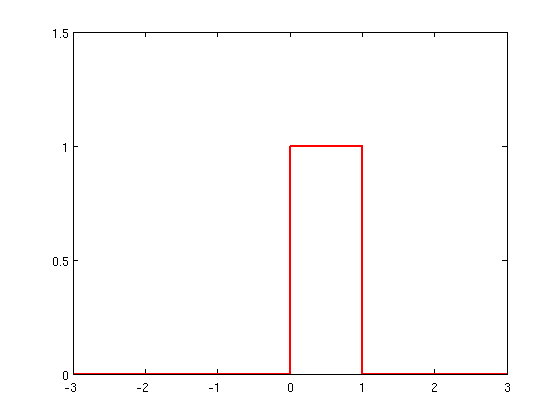
\includegraphics[width=0.5\textwidth]{./images/q2_3a}}
  \subfloat[]{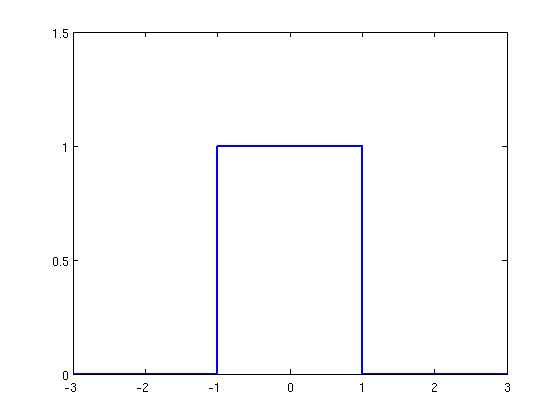
\includegraphics[width=0.5\textwidth]{./images/q2_3b}}
  \caption{Shows the two signals.}
    \label{fig:q2_3a}
\end{figure}

\begin{enumerate}

\item \label{eq:1} $x < -1$
\item \label{eq:2} $-1 \leq x < 0$
\item \label{eq:3} $0 \leq x < 1$
\item \label{eq:4} $1 \leq x < 2$
\item \label{eq:5} $2 \leq x$

\end{enumerate}

If we consider case \ref{eq:1} and \ref{eq:5} these are easy, because there is no overlap between the functions and therefore the convolution is $0$.

\begin{equation*}
  \int_{-\infty}^{-1} {f(\alpha)g(x - \alpha)} d\alpha = \int_{2}^{\infty} {f(\alpha)g(x - \alpha)} d\alpha = 0
\end{equation*}

Next we consider case \ref{eq:2} this is where the functions starts to
overlap, this means that the convolution will generate a linear line from $0$--$AB$.

\begin{equation*}
  \int_{-1}^{x} AB d\alpha = AB \int_{-1}^{x} 1 d\alpha = AB[\alpha]_{-1}^{x} =AB(x + 1)
\end{equation*}

Case \ref{eq:3} is also pretty trivial, the convolution of $0$--$1$ results in a constant function of $AB$ with length $1$.

\begin{equation*}
  \int_{0}^{1} AB d\alpha = AB \int_{0}^{1} 1 d\alpha = AB
\end{equation*}

The last case \ref{eq:4} is the descent from $AB$ down to $0$ again as a linear line.

\begin{equation*}
  \int_{x}^{2} AB d\alpha = AB \int_{x}^{2} 1 d\alpha = AB[\alpha]_{x}^{2} = AB(2 - x)
\end{equation*}

\begin{equation*}
  (g \convolution f)(x) = \begin{cases}
    0 & \textrm{if } x < -1 \\
    AB(x+1) & \textrm{if } -1 \leq x < 0 \\
    AB & \textrm{if } 0 \leq x < 1 \\
    AB(2-x) & \textrm{if } 1 \leq x < 2 \\
    0 & \textrm{if } 2 \leq x
    \end{cases}
\end{equation*}

Figure \ref{fig:q2_3c} shows the result of the convolution of the two
results, again the result is not $1$, but the product of $AB$.

\begin{figure}[!ht]
  \centering
  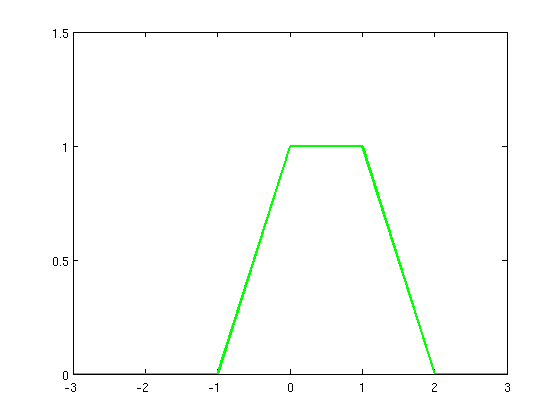
\includegraphics[width=0.7\textwidth]{./images/q2_3c}
  \caption{Shows the convolution of the two signals.}
    \label{fig:q2_3c}
\end{figure}

\subsection*{Question 2.4}

We are to perform convolution on $h(x) = [\nicefrac{1}{3}, \nicefrac{1}{3}, \nicefrac{1}{3}]$ one, two and three times.

\begin{figure}[!ht]
  \centering
  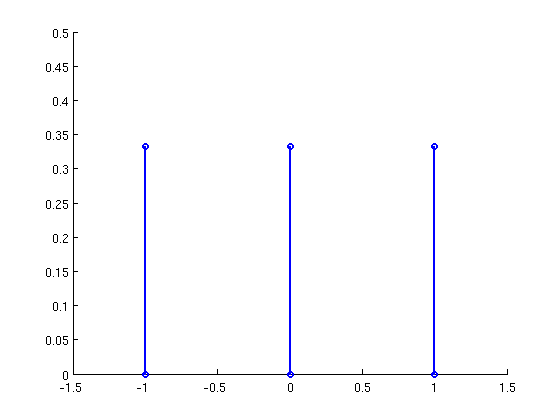
\includegraphics[width=0.7\textwidth]{./images/q2_4a}
  \caption{Shows the convolution of the two signals.}
    \label{fig:q2_4a}
\end{figure}

Figure \ref{fig:q2_4a} shows the original discrete function $h(x)$

Below are shown the results of the convolutions.
\begin{align*}
h_{1}(x) = (h \convolution h)(x) & = \left[ \frac{1}{9}, \frac{2}{9},\frac{3}{9},\frac{2}{9},\frac{1}{9} \right] \\
h_{2}(x) = (h \convolution h_1)(x) & = \left[ \frac{1}{27}, \frac{3}{27},\frac{6}{27},\frac{7}{27},\frac{6}{27}, \frac{3}{27}, \frac{1}{27} \right] \\
h_{3}(x) = (h \convolution h_2)(x) & = \left[ \frac{1}{81}, \frac{4}{81},\frac{10}{81},\frac{16}{81},\frac{19}{81}, \frac{16}{81}, \frac{10}{81}, \frac{4}{81}, \frac{1}{81} \right]
\end{align*}

The length of the resulting signal increases by $2$ with every additional convolution.

\begin{figure}[H]
  \centering
  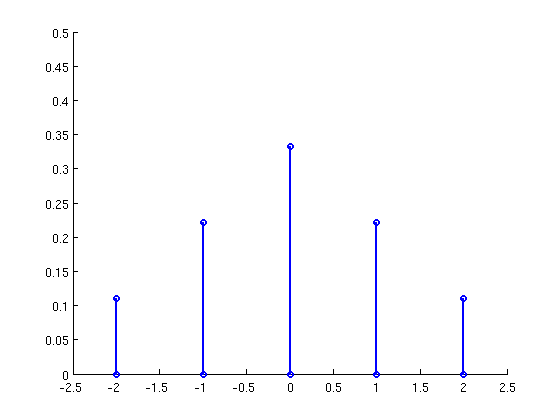
\includegraphics[width=0.7\textwidth]{./images/q2_4b}
  \caption{Shows the $1^{\textrm{st}}$ convolution of the signal.}
    \label{fig:q2_4b}
\end{figure}

Figure \ref{fig:q2_4b} shows the convolution of $h(x)$ with it self, this is $h_1(x)$.

\begin{figure}[H]
  \centering
  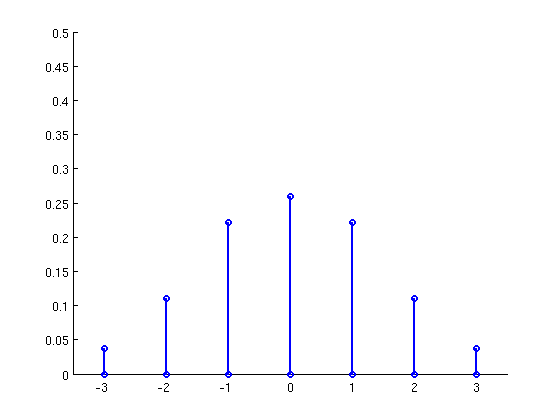
\includegraphics[width=0.7\textwidth]{./images/q2_4c}
  \caption{Shows the $2^{\textrm{nd}}$ convolution of the signal.}
    \label{fig:q2_4c}
\end{figure}

Figure \ref{fig:q2_4c} shows the $2^{\textrm{nd}}$ convolution of
$h(x)$ with it self, this is $h_2(x)$. The shape is now starting to
resemble the something we know, we'll return to this after the next
figure.

\begin{figure}[H]
  \centering
  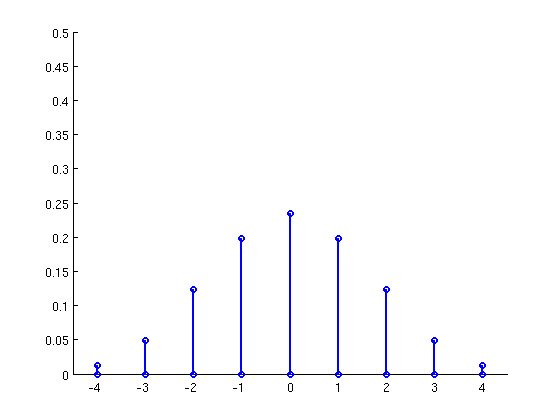
\includegraphics[width=0.7\textwidth]{./images/q2_4d}
  \caption{Shows the $3^{\textrm{rd}}$ convolution of the signal.}
    \label{fig:q2_4d}
\end{figure}

Figure \ref{fig:q2_4d} shows the $3^{\textrm{rd}}$ convolution of
$h(x)$ with it self, this is $h_3(x)$. It is now obvious that the
shape is starting to look like the gaussian distribution. And $(h
\convolution h)^n$ and considering $n \rightarrow \infty$ results in
the gaussian distribution.

%%%%%%%%%%%%%%%%%%%%%%%%%%%%%%%%%%%%%%%%%%%%%%%%%%%%%%%%%%%%%%%%%%%%
% Formal stuff

%\bibliographystyle{abbrvnat}
%\bibliography{bibliography}
%\addcontentsline{toc}{chapter}{Litteratur}

\end{document}

% vim: set tw=72 spell spelllang=en:
